% Multiple Choice Question 7

\begin{center}
    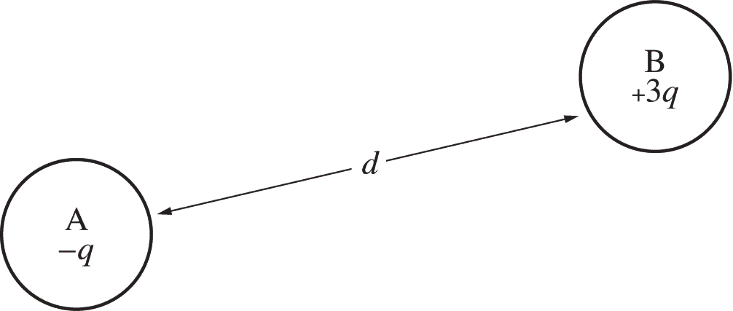
\includegraphics[scale=0.3]{images/img-005-004.png}
\end{center}

\begin{questions}
\setcounter{question}{6}

\question
Conducting spheres A and B of charges $-q$ and $+3q$, respectively, are separated by a distance $d$, as shown in the figure above.
Which of the following statements is true about the two spheres?

\begin{choices}
    \choice The magnitude of the force sphere A exerts on sphere B is three times larger than the magnitude of the force sphere B exerts on sphere A.
    \choice The magnitude of the force sphere B exerts on sphere A is three times larger than the magnitude of the force sphere A exerts on sphere B.
    \choice The force sphere B exerts on sphere A is equal in magnitude to the force sphere A exerts on sphere B.
    \choice If the spheres are free to move, the magnitude of the force sphere B exerts on sphere A will decrease as the spheres move.
    \choice If the spheres are brought into contact with each other and then returned to the positions shown, the two spheres will attract each other.
\end{choices}

\end{questions}
